\documentclass[11pt]{article}
\usepackage[margin=1in]{geometry}
\usepackage{times}
\usepackage{hyperref}
\usepackage{url}
\usepackage{amsmath}
\usepackage{titlesec}
\usepackage{microtype}
\usepackage{parskip}
\usepackage{graphicx}
\usepackage{booktabs}
\usepackage{enumitem}
\usepackage{float}

\setlength{\parindent}{0em}
\setlength{\parskip}{5pt}

\titleformat{\section}{\normalfont\large\bfseries}{\thesection.}{0.5em}{}
\titleformat{\subsection}{\normalfont\normalsize\bfseries}{\thesubsection}{0.5em}{}
\titlespacing*{\section}{0pt}{10pt}{4pt}
\titlespacing*{\subsection}{0pt}{6pt}{3pt}

\title{\textbf{inMediaVeritas: A Decentralized News Verification\\
DApp Using zk-SNARKs and Blockchain Consensus}}

\author{
  inMediaVeritas Group Project\\
  \small{Bc.~Jakub~Ivácek,
  Bc.~Patrik~Baran,
  Bc.~Tomáš~Tisovský,
  Bc.~Vojtech~Babinský,}\\
  \small{Bc.~Tomáš~Miština,
  Bc.~Matúš~Hrkeľ,
  Ing.~Richard~Gazdík,
  doc.~Ing.~Ivan~Homoliak,~Ph.D.}
}

\date{}

\begin{document}

\maketitle
\thispagestyle{empty}

% ----------------------------------------------------------------
\begin{abstract}
\noindent
The proliferation of misinformation in digital media demands trustworthy,
censorship-resistant verification mechanisms that operate without relying on
any central authority. This paper presents \textit{inMediaVeritas}, a
blockchain-based decentralized application (DApp) designed to restore public
trust through a three-tier architecture involving verified reporters, community
witnesses, and news agencies. The system leverages zk-SNARKs for
privacy-preserving location verification, IPFS for decentralized media storage,
and on-chain consensus to collectively establish event truthfulness. Beyond the
core verification pipeline, we describe three companion applications developed
as part of the system: an identity wallet for reporters and witnesses, a
simplified authority application for credential issuers, and a news agency
subscription interface. We detail the system architecture, cryptographic
mechanisms, incentive design, implementation experience, and key limitations.
\end{abstract}

\textbf{Keywords:} blockchain, zk-SNARKs, decentralized verification,
misinformation, IPFS, Ethereum, digital identity, news provenance

% ----------------------------------------------------------------
\section{Introduction}


The rapid and largely unchecked spread of false information across digital
platforms poses a systemic threat to democratic institutions, public health
discourse, and social cohesion~\cite{lazer2018}. Traditional fact-checking
pipelines depend on centralized intermediaries—editorial boards, platform
algorithms, or designated verification services which introduce single points
of failure, susceptibility to political or commercial bias, and a fundamental
asymmetry of trust: users must accept the authority of the verifier without
independent recourse.

Decentralized technologies offer a meaningful alternative. By distributing the
verification burden across a network of economically incentivized participants
whose behavior is governed by cryptographically enforced smart contracts,
it becomes possible to construct a verification system that no single party
can capture, censor, or manipulate. The blockchain's immutability provides
a permanent, auditable record of every submission, vote, and consensus outcome,
while zero-knowledge proofs allow participants to assert facts about themselves
(such as their physical proximity to an event) without exposing private data.

\textit{inMediaVeritas} applies these ideas to the full news lifecycle.
Reporters upload media with cryptographic proof of their location at the time
of capture. Community members geographically proximate to the event submit
testimonials verified through zk-SNARKs. News agencies then pay subscription
fees to access and license verified, blockchain-attested media. The result is
a pipeline from raw media capture to verified, licensable content that requires
no trusted intermediary to arbitrate truth.

This paper makes the following contributions:
\begin{enumerate}[noitemsep]
  \item A complete three-tier architecture for decentralized news verification
    combining zk-SNARKs, IPFS, and Ethereum smart contracts.
  \item A credibility-weighted witness consensus protocol with slashing
    incentives for dishonest behavior.
  \item Three companion applications: an identity wallet for participants,
    a credential authority application for identity issuers, and a news agency
    subscription and access interface.
  \item A discussion of the practical challenges encountered during
    implementation and the limitations of the current design.
\end{enumerate}

% ----------------------------------------------------------------
\section{Related Work}

\subsection{Automated Fact-Checking}

NLP-based systems such as ClaimBuster~\cite{hassan2017} automate claim
detection and routing to fact-checkers, but are limited by language ambiguity,
domain specificity, and the latency of human review cycles. More recent
large-language-model approaches improve fluency and coverage but remain
susceptible to confident hallucination and do not produce verifiable provenance
records.

\subsection{Blockchain Provenance}

Blockchain-based provenance systems~\cite{hasan2019} provide immutable audit
trails for digital media, establishing that a given artifact existed at a given
time. However, these systems lack community-driven verification of the
\textit{events} depicted in the media: provenance confirms what was recorded,
not whether it is truthful.

\subsection{Zero-Knowledge Proofs}

Zk-SNARKs, introduced to the applied cryptography community most visibly
through Zcash~\cite{bensasson2014} and subsequently extended by the PLONK
proving system~\cite{gabizon2019} or CIRCOM~\cite{circom} circuits, allow a prover to demonstrate knowledge of
a secret witness satisfying a circuit constraint without revealing any
information beyond the validity of the statement. This property is critical for
protecting the physical locations of journalists and witnesses operating in
sensitive or dangerous environments.

\subsection{Decentralized Storage}

IPFS~\cite{benet2014} provides content-addressed, censorship-resistant media
storage. Content is identified by its cryptographic hash, meaning any
modification to a media artifact produces a different identifier—making
tampering immediately detectable.

\subsection{Prior Journalism Platforms}

The Civil platform~\cite{civil2018} combined IPFS with blockchain-based
governance for journalism, but lacked a robust community verification mechanism
and ultimately faced challenges with adoption and token economics.
\textit{inMediaVeritas} addresses both gaps by integrating community witness
voting with cryptographically enforced incentives.

% ----------------------------------------------------------------
\section{System Architecture}

\textit{inMediaVeritas} is organized around three interacting actor tiers.
All persistent state is anchored to a public blockchain (Ethereum or a
compatible L2 network), with media stored on IPFS and referenced by on-chain
content identifier (CID) hashes. 

\begin{figure}[H]
    \centering
    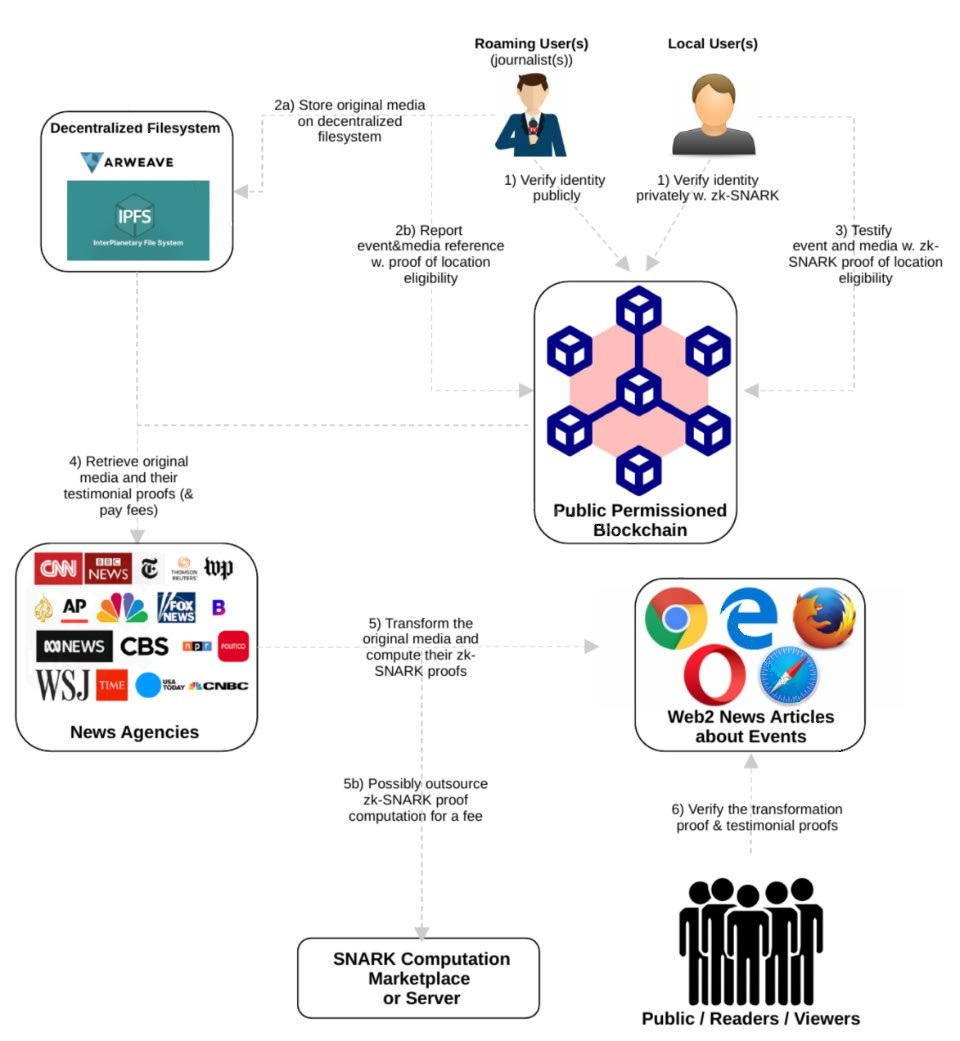
\includegraphics[width=0.8\textwidth]{tp.jpg}
    \caption{Architecture overview.}
    \label{fig:my_label}
\end{figure}
\newpage
\subsection{Reporter Layer}

Reporters are credentialed participants whose real-world identities are verified
through a decentralized identity (DID) registry prior to their first submission.
Each news submission bundles three elements committed atomically on-chain via a
smart contract: a media artifact stored on IPFS and referenced by its CID, a precise timestamp, and a
SHA-256 integrity hash of the raw media. Reporters stake reputation tokens at
submission time; demonstrated misconduct triggers slashing, creating a direct
economic disincentive for fabricated or misleading reports.

\subsection{Witness Layer}

Community witnesses are users who are geographically proximate to a reported
event. Each witness submits a testimonial (confirm or deny) accompanied by a
zk-SNARK proof that their location at the time of the event falls within the
claimed event radius, without revealing their precise coordinates. Witness votes
are weighted by each witness's historical \textit{credibility score}, which is
derived from the alignment of their past votes with the eventual consensus
outcomes of resolved events. This mechanism rewards accurate and honest
engagement over time, and discourages both coordinated brigading and
indiscriminate voting.

The witness contract enforces a minimum quorum before any event is resolved.
If quorum is not reached within a configurable time window, the event is marked
as unresolved and the reporter's stake is returned. Resolved events are
permanently recorded on-chain with the aggregate credibility-weighted vote
outcome.

\subsection{News Agency Layer}

News agencies access verified media and the associated on-chain attestation
records by purchasing weekly, monthly, or yearly subscription plans.
Subscription fees flow into a shared protocol pool that funds reporter
submissions and witness votes, ensuring the system is economically
self-sustaining without external grants or centralized governance. Agencies
also receive cryptographic proofs, generated on demand, confirming that any
published artifact is unaltered and that the associated on-chain record is
authentic.

The news agency interface provides subscribing organizations with a dashboard
for discovering, filtering, and licensing verified content. Agencies can search
the on-chain event registry by location, time range, topic tags, and consensus
confidence score. For each event, the interface displays the associated media,
the full witness vote breakdown, and a downloadable cryptographic proof of
authenticity suitable for inclusion in published reporting. Subscription
management, including plan selection and renewal, is handled through a
straightforward web front-end that interacts with the subscription smart contract.

% ----------------------------------------------------------------
\section{Companion Applications}

In addition to the core smart contract infrastructure, three companion
applications were developed to make the system accessible to non-technical
participants and to complete the end-to-end user flow.

\subsection{Identity Wallet}

The identity wallet is a mobile-first application through which reporters and
witnesses manage their decentralized identities and interact with the
\textit{inMediaVeritas} protocol. It is inspired by EUDI/EIDAS standard for identity wallets in the EU. No suitable existing solution was found, thus it was decided to create a custom tailored application that suits needs of this project. Its primary functions are:

\begin{itemize}[noitemsep]
  \item \textbf{Credential storage}: Holding verifiable credentials issued by
    the authority application (described below), which attest to the user's
    registration status as a reporter or witness.
  \item \textbf{Submission and voting}: Allowing reporters to compose and submit
    news events capturing media, attaching a location commitment, and signing
    the transaction and allowing witnesses to cast credibility-weighted votes
    with automatically generated zk-SNARK location proofs.
    \item \textbf{Biometric-Protected Signing}: Rather than requiring users to manually manage 256-bit private keys, the app utilizes \textit{react-native-biometrics}. This allows users to sign protocol messages (reports, votes, and registrations) using keys stored in the device's Secure Enclave or Keystore, triggered by FaceID or Fingerprint.\textbf{}
\end{itemize}


\subsection{Authority Application}

The authority application is a simplified web interface for credential issuers
(such as governmental bodies or trusted news organizations) who are responsible
for verifying the real-world identities of reporters and witnesses before
admitting them to the protocol. Its functions include:

\begin{itemize}[noitemsep]
  \item \textbf{Identity verification}: Reviewing submitted government-issued
    credential proofs and approving or rejecting applicants.
  \item \textbf{Credential issuance}: Issuing signed verifiable credentials to
    approved participants, which are then stored in their identity wallets and
    presented when required by the smart contract.
  \item \textbf{Audit log}: Maintaining a tamper-evident log of all issuance
   actions.
\end{itemize}

The authority application is deliberately minimal by design: its role is to
bootstrap trust at the identity layer without becoming a bottleneck or a
central point of control over content decisions. In the future multiple authority applications can be used, (each government can have its own solution) but they all have to support API for communication with the ID app.


% ----------------------------------------------------------------
\section{Cryptographic Mechanisms}

\subsection{Zero-Knowledge Location Proofs}

The core privacy primitive is a zk-SNARK circuit that accepts a witness's
location and their DID-linked identity commitment as private
inputs, and proves that (i) the location falls within the declared event
radius, and (ii) the identity commitment corresponds to a registered
participant, without revealing either the exact location or the underlying
identity. We implement this circuit using the CIRCOM proving system~\cite{circom}
over the Baby JubJub elliptic curve~\cite{babyjubjub}—a curve natively
optimized for efficient arithmetic inside zk-SNARK circuits and for Ethereum
verification. Proof generation runs in a few seconds on consumer hardware;
on-chain verification is performed by a Solidity verifier contract generated
from the circuit's verification key.

\subsection{Media Integrity}

All uploaded media is SHA-256 hashed client-side before upload and the hash
is committed on-chain at submission time, creating an immutable fingerprint of
the original content. The IPFS CID independently encodes the content hash of
the stored artifact. Together, these two independent integrity checks ensure
that any tampering with the media after submission is immediately detectable by
any party with access to the original artifact.

\subsection{Verifiable Credentials and Identity}

Reporter and witness identities are anchored to Identity Credentials, each linked to a government-issued credential via a zero-knowledge
credential proof. This proof demonstrates that the holder possesses a valid
government-issued identity document without revealing the document's contents
or the holder's name or address. Credentials are issued by registered authority
nodes and stored in participants' identity wallets. The smart contract verifies
credential validity on-chain before accepting submissions or votes.

% ----------------------------------------------------------------
\section{Incentive Model}

\textit{inMediaVeritas} is designed to be economically self-sustaining. News
agency subscription fees flow into a shared protocol pool, from which:
(i)~reporters receive a gas reimbursement and a small reward upon successful
event resolution, (ii)~witnesses receive a proportional share of the resolution
reward based on their credibility-weighted contribution to the correct consensus,
and (iii)~stakes are slashed from dishonest participants and redistributed to
the pool.

This design creates a virtuous cycle: agency demand for verified content
directly funds the participation of reporters and witnesses, who are in turn
incentivized to report accurately and vote honestly. No external funding source,
governance token, or centralized treasury is required to sustain the system.

A key design choice is that reporters and witnesses are not required to provide
their own capital. The protocol pool pre-funds participation costs, lowering
the barrier to entry for individual contributors. Slashing applies only to
pre-funded stakes, not to personal funds, preventing punitive outcomes for
good-faith participants who encounter edge cases.

% ----------------------------------------------------------------
\section{Implementation}

The system was implemented as a proof-of-concept targeting the Ethereum Sepolia
testnet. Smart contracts were written in Solidity and deployed using Hardhat.
The zk-SNARK circuits were implemented using the Circom language and compiled
with the SnarkJS toolchain, which also generated the Solidity verifier contract.
IPFS storage was integrated via the Helia library.

The identity wallet was built as a React Native application,
deployment on Android smartphones. The authority application was implemented as a
standard React web application. Both front-ends interact with the blockchain
via ethers.js and with the IPFS node via the Helia HTTP API.


% ----------------------------------------------------------------
% ----------------------------------------------------------------
\section{Evaluation}

We evaluated the key performance characteristics of the \textit{inMediaVeritas}
proof-of-concept. On-chain gas costs were measured on a local EVM (the Remix
JavaScript VM), which executes identical bytecode and charges identical gas to
a public network such as Sepolia; the measured values are therefore
representative of mainnet/testnet execution. zk-SNARK proof generation was
measured using the SnarkJS CLI.

\subsection{Experimental Setup}

On-chain gas measurements were performed on the Remix VM
(Solidity~0.8.13, optimizer enabled, \texttt{runs}=200, \texttt{viaIR}=true).
zk-SNARK proof generation was measured with SnarkJS~v0.7.6 (Node.js~20.17.0)
using the Groth16 proving system on the following platform:
\begin{itemize}[noitemsep]
  \item \textbf{Desktop}: AMD Ryzen~5 7600X (6~cores / 12~threads, 4.7~GHz),
        32~GB RAM, Windows~11 with WSL~2 (Ubuntu).
\end{itemize}
The proving curve is BN254 (alt\_bn128); the Baby JubJub curve is used only as
the embedded curve inside the circuits.

\subsection{zk-SNARK Proof Generation}

The identity circuit is compiled with the Groth16 proving scheme and contains
approximately 7\,680 arithmetic constraints.
Table~\ref{tab:snark} reports witness generation and proof generation times.
The final Groth16 proof is 192~bytes and is submitted on-chain as part of the
\texttt{voteOnMediaWithProof} transaction.

\begin{table}[ht]
\centering
\small
\caption{zk-SNARK proof generation time (Groth16, cold run, SnarkJS~v0.7.6).}%
\label{tab:snark}
\begin{tabular}{lrrr}
\toprule
Circuit & Witness gen.\ (s) & Proof gen.\ (s) & Total (s) \\
\midrule
Identity & 1.121 & 1.454 & 2.575 \\
Location & 0.951 & 1.411 & 2.362 \\
\bottomrule
\end{tabular}
\end{table}

The reported times correspond to a cold run, in which the dominant component is
Node.js startup (approximately 0.9~s); the cryptographic work itself accounts
for under 0.5~s. In a production setting with a long-running Node process this
overhead is amortised, reducing proof generation to an estimated 0.3--0.5~s per
proof. Repeated proving within the same session likewise benefits from the
operating system file cache. The two circuits exhibit similar costs, consistent
with their comparable constraint counts; the location circuit is marginally
faster despite producing a larger public input vector. The measurements were
obtained on a high-performance desktop CPU; on weaker laptop-class hardware the
same circuits are expected to take several seconds per cold proof, which remains
acceptable for an interactive client-side proving workflow.

Circuit setup (Table~\ref{tab:setup}) is performed only once per circuit; every
subsequent proof requires only witness calculation and proving.

\begin{table}[ht]
\centering
\small
\caption{One-time circuit setup cost (performed once per circuit).}%
\label{tab:setup}
\begin{tabular}{lrr}
\toprule
Phase & Identity (s) & Location (s) \\
\midrule
Circom compilation (r1cs + wasm) & 1.872 & 1.811 \\
Groth16 setup (zkey)             & 4.877 & 4.419 \\
zkey contribution                & 1.675 & 1.704 \\
\midrule
Total setup                      & 8.424 & 7.934 \\
\bottomrule
\end{tabular}
\end{table}

\subsection{On-Chain Gas Costs}

Table~\ref{tab:gas} reports the gas consumed by each state-changing protocol
operation. At a reference gas price of 10~gwei the corresponding ETH cost per
call is also shown. View functions (e.g.\ \texttt{getEvent},
\texttt{getMediaItem}) are omitted, as they incur no gas when called off-chain.

Three effects are visible in the data. First, the cost of \texttt{createEvent}
scales approximately linearly with the number of attached media items
($\approx$150--170k gas per item), reflecting the on-chain storage of media
metadata strings. Second, voting cost depends on storage warmth: the first vote
on a given event initialises its counters from zero (cold
$0\rightarrow1$ storage writes, $\approx$20k gas each), whereas a subsequent
vote on the same event updates already-nonzero counters at a reduced cost,
lowering the per-vote cost from $\approx$95k to $\approx$61k gas. Third, the
\texttt{isLocalVoter} flag adds the cost of one additional counter update: when
set, the vote increments a separate local-tally counter, and initialising that
counter from zero adds a further $\approx$20k gas. This explains why the two
\texttt{voteOnMedia} measurements differ in the opposite direction to
\texttt{voteOnEvent}: the first \texttt{voteOnMedia} call was cast with
\texttt{isLocalVoter} disabled (76\,190~gas), while the second enabled it,
incurring the additional cold local-counter write (81\,307~gas).

\begin{table}[ht]
\centering
\small
\caption{Gas consumption per protocol operation (Remix VM, Solidity 0.8.13, optimizer on).}%
\label{tab:gas}
\begin{tabular}{lrr}
\toprule
Operation & Gas (units) & ETH at 10~gwei \\
\midrule
Contract deployment                       & 1\,649\,455 & 0.016495 \\
\texttt{createEvent} (0 media)            &   280\,774 & 0.002808 \\
\texttt{createEvent} (1 media)            &   450\,615 & 0.004506 \\
\texttt{createEvent} (3 media)            &   735\,659 & 0.007357 \\
\texttt{addMediaItem}                     &   212\,567 & 0.002126 \\
\texttt{voteOnEvent} (first, local)       &    95\,533 & 0.000955 \\
\texttt{voteOnEvent} (subsequent, local)  &    61\,333 & 0.000613 \\
\texttt{voteOnMedia} (first, non-local)   &    76\,190 & 0.000762 \\
\texttt{voteOnMedia} (subsequent, local)  &    81\,307 & 0.000813 \\
\bottomrule
\end{tabular}
\end{table}

\subsection{zk-Enabled Voting Cost}

The figures in Table~\ref{tab:gas} correspond to the non-zk (demonstration)
voting mode, in which the voter hash and locality flag are supplied directly.
In the zk-enabled mode, a vote is submitted via \texttt{voteOnMediaWithProof},
whose cost is the sum of the storage-update cost measured above ($\approx$76k
gas) and the cost of on-chain Groth16 proof verification performed by the
verifier contract.

The verification cost was measured by deploying the SnarkJS-generated Solidity
verifier (via \texttt{snarkjs zkey export solidityverifier}) for each circuit
and submitting a real proof produced by the proving pipeline. Both proofs
verified successfully on-chain. Table~\ref{tab:zkverify} reports the measured
verification cost; the figures correspond to the EVM execution cost, which is
the relevant quantity when \texttt{verifyProof} is invoked internally by
\texttt{voteOnMediaWithProof} rather than as a standalone transaction.

\begin{table}[ht]
\centering
\small
\caption{On-chain Groth16 proof verification cost (Remix VM, BN254 curve).}%
\label{tab:zkverify}
\begin{tabular}{lrr}
\toprule
Circuit & Public inputs & \texttt{verifyProof} gas \\
\midrule
Identity & 5 & 214\,787 \\
Location & 7 & 227\,978 \\
\bottomrule
\end{tabular}
\end{table}

As expected for Groth16 on the BN254 curve, verification is dominated by the
three elliptic-curve pairing operations and is largely independent of the
circuit's internal size; the small difference between the two circuits
($\approx$13k gas) reflects the two additional public inputs of the location
circuit, each of which adds one scalar multiplication to the linear combination
of the verification key ($\approx$6.5k gas per input).

Combining these results, the end-to-end cost of a zk-enabled media vote is
approximately $214\,787 + 76\,190 \approx 291\,000$~gas for the identity circuit
(and $227\,978 + 76\,190 \approx 304\,000$~gas for the location circuit), of
which proof verification accounts for roughly 74\,--\,75\%. On-chain proof
verification, rather than state storage, is therefore the dominant cost in the
privacy-preserving voting path. At a reference gas price of 10~gwei this
corresponds to approximately $0.0029$~ETH per zk-enabled vote.
% ----------------------------------------------------------------
% ----------------------------------------------------------------
\section{Discussion and Limitations}

\textit{inMediaVeritas} demonstrates that a fully decentralized, privacy-preserving
news verification pipeline is technically feasible. However, several limitations
merit acknowledgment.

\textbf{Sparse witness coverage.} The system's correctness depends on a
sufficient number of geographically proximate witnesses being present and
willing to vote. In low-density areas, rural regions, or for events occurring
at unusual times, quorum may be difficult to reach. Mechanisms for incentivizing
proactive witness registration in underserved areas remain an open problem.

\textbf{Authority centralization risk.} While multiple authorities can operate
in parallel, the credential issuance step reintroduces a degree of centralization
at the identity layer. A malicious or captured authority could exclude legitimate
reporters or admit Sybil accounts. Federated authority governance and
cross-authority credential recognition are mitigations under consideration.

\textbf{Legal and regulatory uncertainty.} The legal landscape for decentralized
media licensing is nascent, and smart contract fee enforcement may conflict with
jurisdictional copyright, data protection, or media liability frameworks.
Production deployment would require careful legal analysis across target
jurisdictions.

\textbf{Scalability.} The current implementation targets a single Ethereum L1
or L2 deployment. High-volume news cycles breaking events with thousands of
concurrent submissions would stress both the contract gas costs and the IPFS
pinning infrastructure. Layer-2 rollups and sharded IPFS pinning clusters are
natural directions for scaling.

% ----------------------------------------------------------------
\section{Conclusion}

This paper presented \textit{inMediaVeritas}, a decentralized application
addressing the misinformation crisis through cryptographic verification,
community consensus, and transparent provenance. By combining zk-SNARK location
proofs, IPFS media storage, blockchain immutability, credibility-weighted witness
voting, and a carefully designed self-sustaining incentive layer,
\textit{inMediaVeritas} enables a trustless pipeline from raw media capture to
verified, licensable content without relying on any central authority to
arbitrate truth.

The companion identity wallet, authority application, and news agency interface
demonstrate that the core protocol can be made accessible to non-technical
participants across all three tiers of the system. While significant engineering
and sociotechnical challenges remain before production deployment, the proof-of-concept
validates the architectural approach and identifies a concrete roadmap for future
work.

% ----------------------------------------------------------------
\begin{thebibliography}{99}
\small

\bibitem{lazer2018}
Lazer, D. M. J., et al. \textit{The science of fake news}. Science, 359(6380), 1094--1096, 2018.

\bibitem{hassan2017}
Hassan, N., et al. \textit{ClaimBuster: The first-ever end-to-end fact-checking system}. PVLDB, 10(12), 2017.

\bibitem{hasan2019}
Hasan, H. R., \& Salah, K. \textit{Combating deepfake videos using blockchain and smart contracts}. IEEE Access, 7, 2019.

\bibitem{bensasson2014}
Ben-Sasson, E., et al. \textit{Zerocash: Decentralized anonymous payments from Bitcoin}. IEEE S\&P, 2014.

\bibitem{gabizon2019}
Gabizon, A., et al. \textit{PLONK: Permutations over Lagrange-bases for oecumenical noninteractive arguments of knowledge}. IACR ePrint 2019/953.

\bibitem{circom}
M. Bellés-Muñoz, M. Isabel, J. L. Muñoz-Tapia, A. Rubio and J. Baylina, "Circom: A Circuit Description Language for Building Zero-Knowledge Applications," in IEEE Transactions on Dependable and Secure Computing, vol. 20, no. 6, pp. 4733-4751, Nov.-Dec. 2023, doi: 10.1109/TDSC.2022.3232813.
keywords: {Arithmetic;Wires;Logic gates;Smart contracts;Libraries;Distributed ledger;Program processors;Zero-knowledge proof;circuit;domain-specific language;compiler;blockchain},

\bibitem{benet2014}
Benet, J. \textit{IPFS -- Content addressed, versioned, P2P file system}. arXiv:1407.3561, 2014.

\bibitem{civil2018}
Civil Media Company. \textit{The Civil Cryptoeconomic Whitepaper}, 2018.

\bibitem{babyjubjub}
Bell\'{e}s-Mu\~{n}oz, M., et al. \textit{Twisted Edwards Elliptic Curves for Zero-Knowledge Circuits}. Mathematics, 9(23), 2021.

\end{thebibliography}

\end{document}